%-------------------------
% CV MARIO CELZO - Design Moderno 2 Pagine
%-------------------------

\documentclass[10pt,a4paper]{article}

\usepackage[utf8]{inputenc}
\usepackage[T1]{fontenc}
\usepackage[italian]{babel}
\usepackage[left=0cm, right=0.5cm, top=0cm, bottom=0.5cm]{geometry}
\usepackage{xcolor}
\usepackage{tikz}
\usepackage{fontawesome5}
\usepackage{hyperref}
\usepackage{graphicx}
\usepackage{tabularx}

\usetikzlibrary{calc}

\pagestyle{empty}
\setlength{\parindent}{0pt}

% ============ COLORS ============
\definecolor{primary}{HTML}{2D3748}
\definecolor{accent}{HTML}{3182CE}
\definecolor{sidebar}{HTML}{EDF2F7}
\definecolor{textgray}{HTML}{718096}
\definecolor{success}{HTML}{38A169}
\definecolor{warning}{HTML}{DD6B20}
\definecolor{danger}{HTML}{E53E3E}
\definecolor{purple}{HTML}{805AD5}
\definecolor{pink}{HTML}{D53F8C}
\definecolor{cyan}{HTML}{00B5D8}
\definecolor{yellow}{HTML}{D69E2E}
\definecolor{linkedinblue}{HTML}{0077B5}
\definecolor{githubbg}{HTML}{24292E}
\definecolor{dockerblue}{HTML}{2496ED}

\hypersetup{colorlinks=true, urlcolor=accent}

% ============ COMMANDS ============
\newcommand{\sidebarsection}[2]{%
    \vspace{0.3cm}
    {\normalsize\bfseries\textcolor{primary}{\faIcon{#1}~~#2}}\\[0.08cm]
    {\color{accent}\rule{4.3cm}{1.5pt}}\\[0.12cm]
}

\newcommand{\mainsection}[2]{%
    \vspace{0.25cm}
    {\large\bfseries\textcolor{primary}{\faIcon{#1}~~#2}}\\[0.05cm]
    {\color{accent}\rule{11.5cm}{1.5pt}}\\[0.15cm]
}

\newcommand{\skilltag}[3]{%
    \tikz[baseline=(char.base)]{
        \node[fill=#1!15, text=#1!80!black, rounded corners=3pt, inner sep=3.5pt, font=\scriptsize\bfseries] (char) {\faIcon{#2}~#3};
    }\hspace{0.03cm}
}

\newcommand{\linkbadge}[3]{%
    \tikz[baseline=(char.base)]{
        \node[fill=#1, text=white, rounded corners=2pt, inner sep=2.5pt, font=\tiny\bfseries] (char) {\faIcon{#2}~#3};
    }
}

% Header command per riutilizzo
\newcommand{\cvheader}{%
    % Header background
    \begin{tikzpicture}[remember picture, overlay]
        \fill[primary] (current page.north west) rectangle ([yshift=-3.5cm]current page.north east);
        \fill[accent] ([yshift=-3.5cm]current page.north west) rectangle ([yshift=-3.6cm]current page.north east);
        \fill[sidebar] ([yshift=-3.6cm]current page.north west) rectangle ([xshift=5.3cm]current page.south west);
    \end{tikzpicture}
    
    % Header content
    \begin{tikzpicture}[remember picture, overlay]
        % Foto circolare - centrata verticalmente (ruotata per verticale)
        \node[anchor=center] at ([xshift=2.5cm, yshift=-1.8cm]current page.north west) {
            \begin{tikzpicture}
                \clip (0,0) circle (1.2cm);
                \node[rotate=-90] at (0,0) {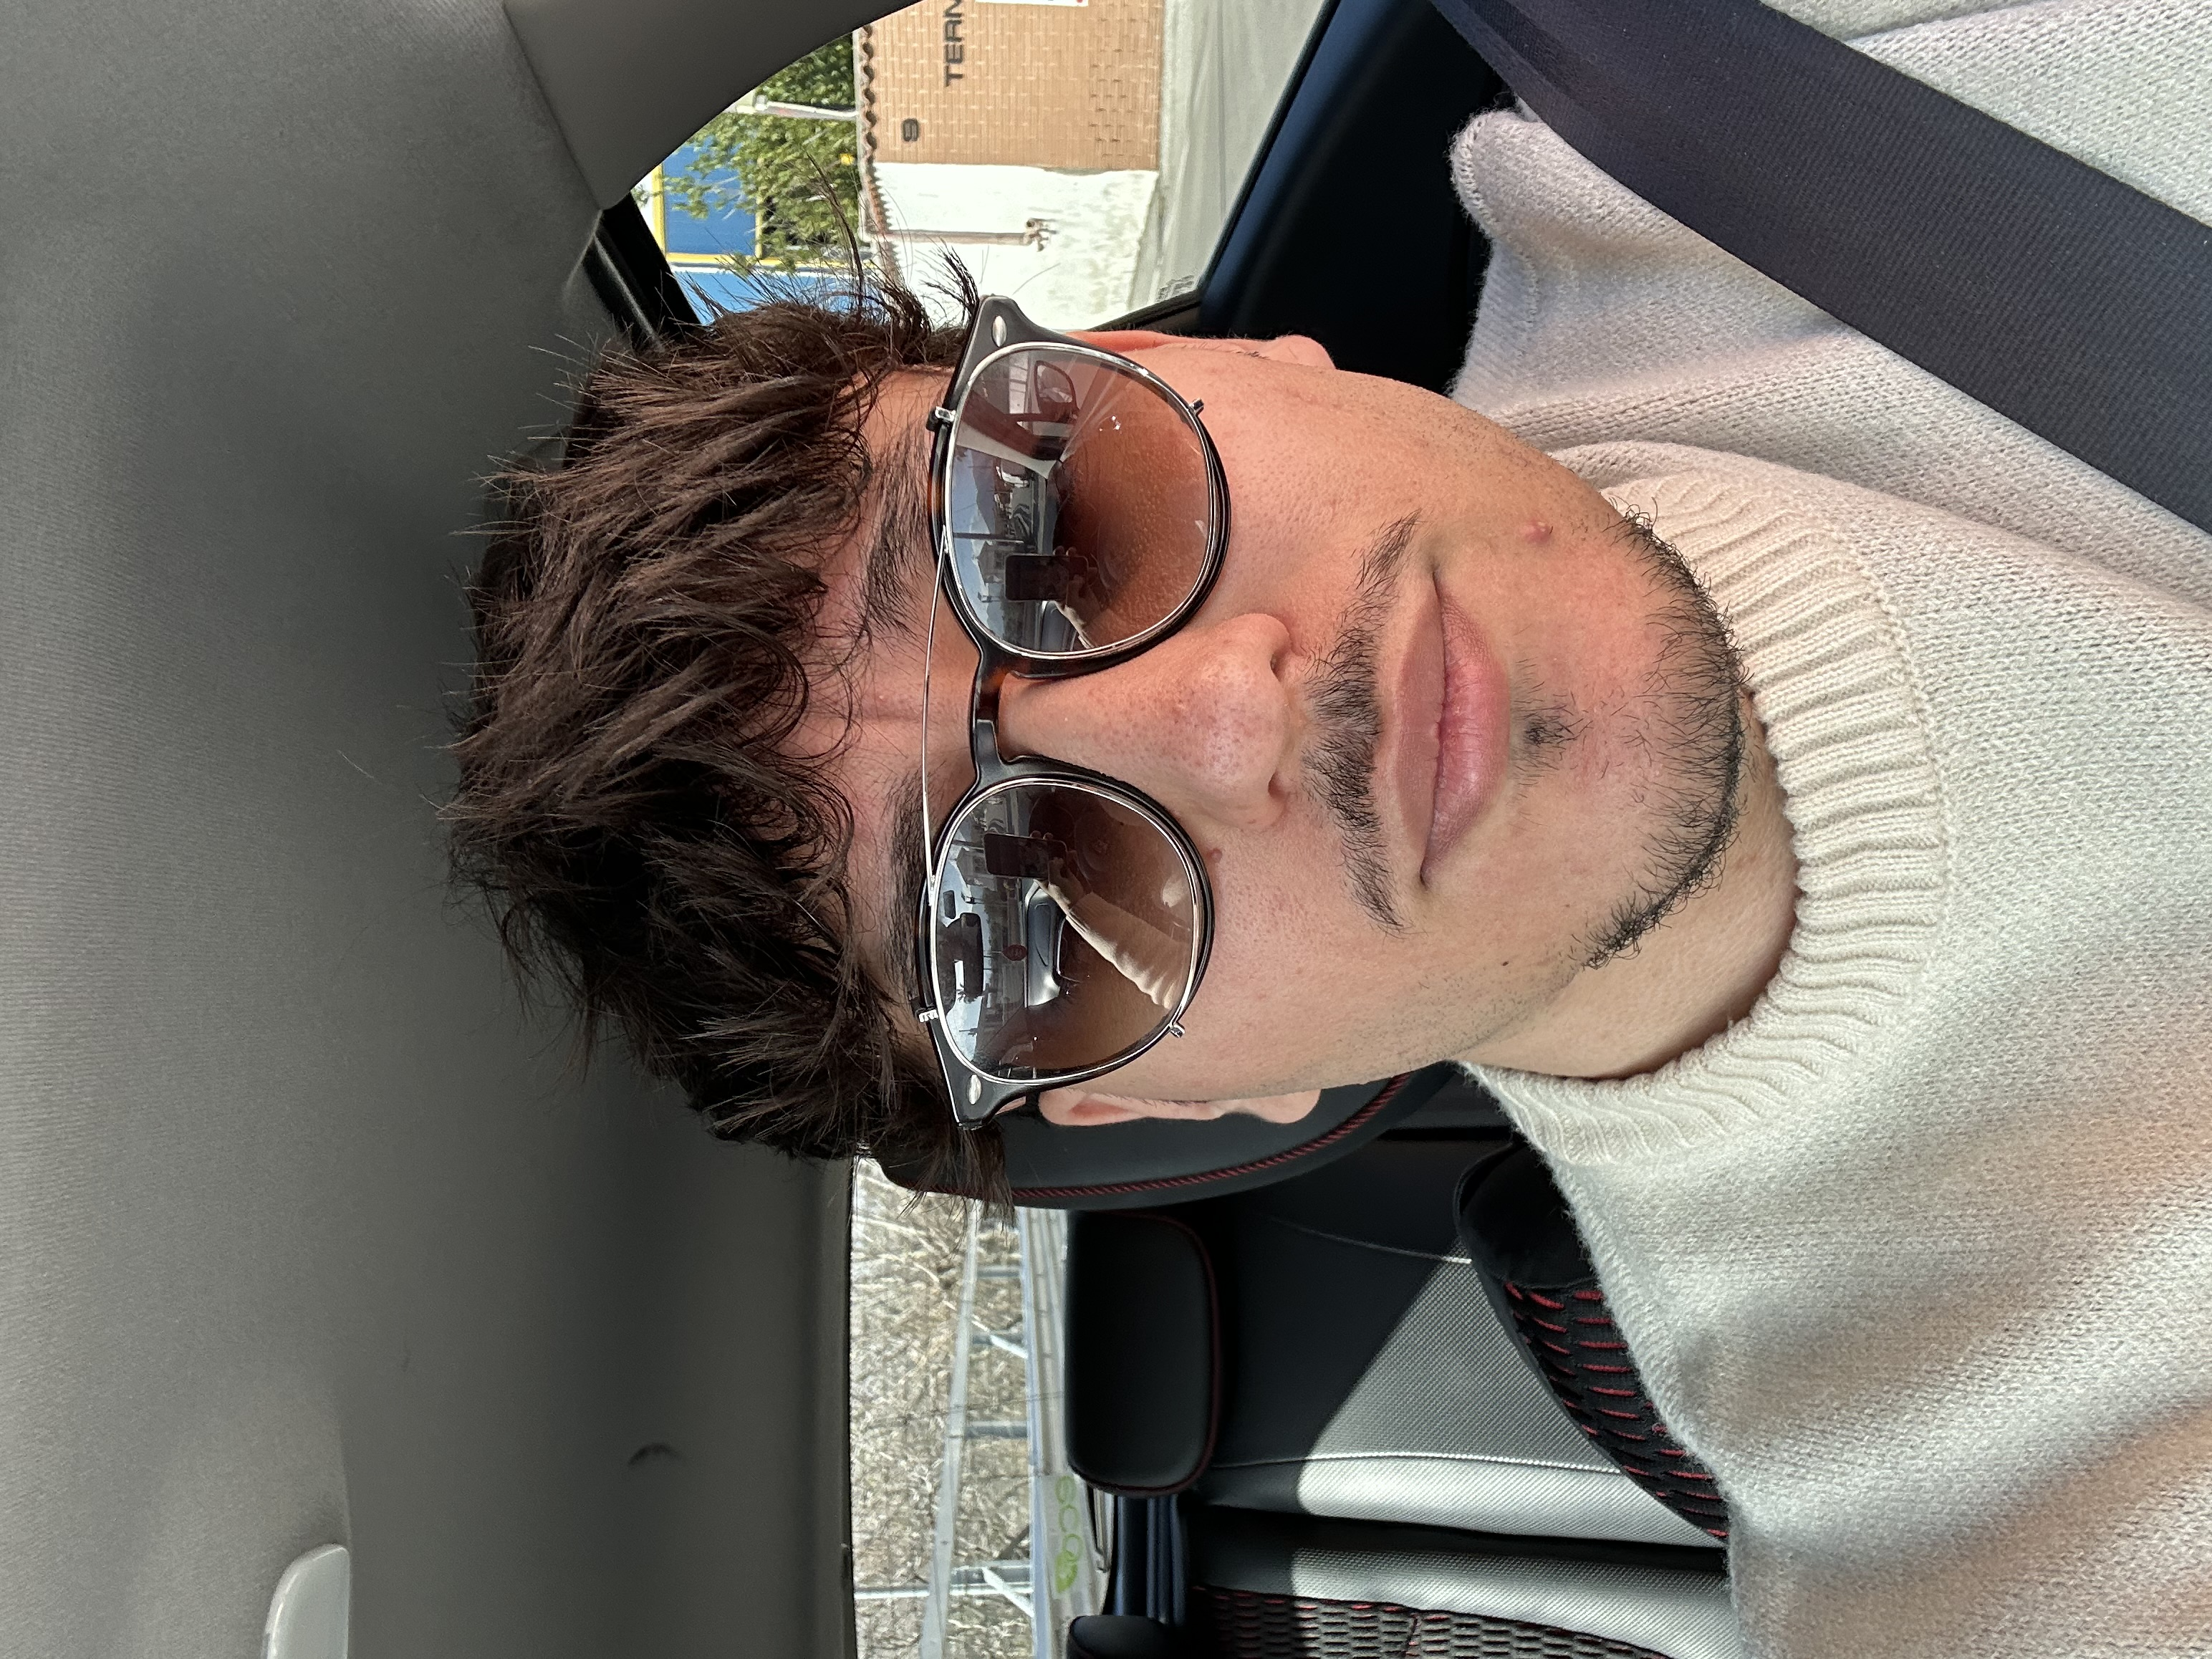
\includegraphics[width=2.4cm]{foto.jpeg}};
                \draw[white, line width=2.5pt] (0,0) circle (1.2cm);
            \end{tikzpicture}
        };
        % Nome
        \node[anchor=west, text=white] at ([xshift=4.5cm, yshift=-1.3cm]current page.north west) {
            {\Huge\bfseries MARIO CELZO}
        };
        % Titolo
        \node[anchor=west, text=white, opacity=0.85] at ([xshift=4.5cm, yshift=-2cm]current page.north west) {
            {\large JUNIOR DEVELOPER / STUDENT}
        };
        % Badge links
        \node[anchor=west] at ([xshift=4.5cm, yshift=-2.8cm]current page.north west) {
            \href{https://mario-celzo.vercel.app}{\linkbadge{accent}{globe}{mario-celzo.vercel.app}}~~%
            \href{https://linkedin.com/in/mario-celzo}{\linkbadge{linkedinblue}{linkedin}{linkedin.com/in/mario-celzo}}~~%
            \href{https://github.com/mariocelzo}{\linkbadge{githubbg}{github}{github.com/mariocelzo}}
        };
    \end{tikzpicture}
    
    \vspace{3.3cm}
}

% ============ DOCUMENT ============
\begin{document}

% ========== PAGE 1 ==========
\cvheader

% Two columns
\noindent
\begin{minipage}[t]{5.3cm}
\hspace{0.4cm}
\begin{minipage}[t]{4.5cm}

\sidebarsection{user}{SU DI ME}
{\footnotesize Laureando in Informatica all'Università di Salerno. La mia priorità è inserirmi nel mondo del lavoro, mettendo in pratica le competenze acquisite e continuando a crescere professionalmente.}

\sidebarsection{address-card}{CONTATTI}
{\footnotesize
\textcolor{success}{\faIcon{phone}}~~+39 3385403836\\[0.1cm]
\textcolor{danger}{\faIcon{envelope}}~~\href{mailto:mariocelzo003@gmail.com}{mariocelzo003@gmail.com}\\[0.1cm]
\textcolor{accent}{\faIcon{map-marker-alt}}~~Sarno (SA), Italia\\[0.1cm]
\textcolor{linkedinblue}{\faIcon{linkedin}}~~\href{https://linkedin.com/in/mario-celzo}{mario-celzo}\\[0.1cm]
\textcolor{githubbg}{\faIcon{github}}~~\href{https://github.com/mariocelzo}{mariocelzo}\\[0.1cm]
\textcolor{purple}{\faIcon{globe}}~~\href{https://mario-celzo.vercel.app}{mario-celzo.vercel.app}
}

\sidebarsection{graduation-cap}{ISTRUZIONE}
{\footnotesize
\textbf{\textcolor{primary}{2025 -- Presente}}\\
Laurea Magistrale in\\Software Engineering \& IT Mgmt\\
{\scriptsize\textcolor{textgray}{Univ. degli Studi di Salerno}}\\[0.15cm]

\textbf{\textcolor{primary}{2022 -- Dic. 2025}}\\
Laurea Triennale in Informatica\\
{\scriptsize\textcolor{textgray}{Univ. degli Studi di Salerno}}\\[0.15cm]

\textbf{\textcolor{primary}{2017 -- 2022}}\\
Diploma Liceo Scientifico\\
{\scriptsize\textcolor{textgray}{Liceo Tito Lucrezio Caro}}
}

\sidebarsection{language}{LINGUE}
{\footnotesize
\textbf{Inglese} -- B2\\
{\scriptsize Ascolto: B2 | Lettura: B1 | Orale: B1-B2}\\[0.1cm]
\textbf{Italiano} -- Madrelingua
}

\sidebarsection{heart}{HOBBY}
{\footnotesize
\textcolor{danger}{\faIcon{flag-checkered}}~Formula 1~~\textcolor{accent}{\faIcon{plane}}~Viaggi\\[0.08cm]
\textcolor{success}{\faIcon{code}}~Coding~~\textcolor{purple}{\faIcon{gamepad}}~Gaming
}

\end{minipage}
\end{minipage}%
\hfill
\begin{minipage}[t]{12.5cm}

\mainsection{rocket}{MY PROJECTS}

\textbf{\textcolor{primary}{TARGET}} \hfill \textcolor{accent}{\small 2024}\\[0.05cm]
{\small Piattaforma e-commerce per compravendita tra privati (stile Vinted/Subito) sviluppata per Ingegneria del Software. Funzionalità: gestione annunci con foto, ricerca avanzata con filtri, chat real-time, sistema recensioni. Team di 3 persone, metodologia Agile/Scrum, forte focus su UX/UI design.}\\[0.08cm]
\href{https://v0-target-svp6klexsij.vercel.app/}{\linkbadge{success}{link}{SITO}}~~\href{https://github.com/mariocelzo/Target}{\linkbadge{githubbg}{github}{GitHub}}

\vspace{0.18cm}

\textbf{\textcolor{primary}{BiblioFlow}} \hfill \textcolor{accent}{\small 2025}\\[0.05cm]
{\small Sistema collaborativo per gestione intelligente biblioteca universitaria (Human Computer Interaction). Analisi ecosistema: prenotazione posti studio con sensori di presenza, prestiti RFID self-service, chatbot per reference desk. Focus su post-human interaction, accessibilità, sostenibilità. Creazione personas, scenari d'uso e prototipi interattivi.}\\[0.08cm]
\href{https://www.figma.com/design/BiblioFlow}{\linkbadge{pink}{figma}{Figma}}

\vspace{0.18cm}

\textbf{\textcolor{primary}{BODY-LIFE}} \hfill \textcolor{accent}{\small 2025}\\[0.05cm]
{\small Applicazione fitness completa per Interazione Uomo-Macchina. Monitoraggio peso corporeo e attività fisica, dashboard interattiva con grafici, workout personalizzati. Processo UX/UI completo: wireframing, prototipazione su Figma, test usabilità. Implementata con React e Next.js.}\\[0.08cm]
\href{https://body-life-teal.vercel.app/}{\linkbadge{accent}{link}{SITO}}~~\href{https://www.figma.com/design/FgrYVoi37erhxvlGQEtiBm/Gym-App--Community-}{\linkbadge{pink}{figma}{Figma}}

\vspace{0.18cm}

\textbf{\textcolor{primary}{NearBite}} \hfill \textcolor{accent}{\small 2025}\\[0.05cm]
{\small App mobile cross-platform (React Native + Expo) per ricerca ristoranti nelle vicinanze. Stack: Supabase per database/auth, Google Places API, geolocalizzazione real-time, sistema raccomandazioni AI. Design moderno con animazioni fluide.}\\[0.08cm]
\href{https://github.com/mariocelzo/resturant-finder}{\linkbadge{githubbg}{github}{GitHub}}

\vspace{0.18cm}

\textbf{\textcolor{primary}{PetClinic Dependability}} \hfill \textcolor{accent}{\small 2025}\\[0.05cm]
{\small Analisi dependability di Spring PetClinic per Software Dependability. Tecniche: fault injection con Chaos Monkey, FMEA, reliability analysis (MTTF/MTTR). Pipeline DevOps: GitHub Actions CI/CD, Docker, quality gate SonarCloud.}\\[0.08cm]
\href{https://github.com/mariocelzo/petclinic-dependability-analysis}{\linkbadge{githubbg}{github}{GitHub}}

\vspace{0.15cm}

\mainsection{code}{SKILLS}

{\small\textbf{Linguaggi \& Framework}}\\[0.08cm]
\skilltag{yellow}{python}{Python}
\skilltag{yellow}{js-square}{JavaScript}
\skilltag{danger}{java}{Java}
\skilltag{cyan}{react}{React}
\skilltag{cyan}{react}{React Native}
\skilltag{danger}{angular}{Angular}

\vspace{0.1cm}
\skilltag{primary}{node-js}{Next.js}
\skilltag{cyan}{mobile-alt}{Flutter}
\skilltag{accent}{database}{SQL}
\skilltag{yellow}{code}{JQuery}

\vspace{0.18cm}
{\small\textbf{DevOps \& Tools}}\\[0.08cm]
\skilltag{githubbg}{git-alt}{Git}
\skilltag{dockerblue}{docker}{Docker}
\skilltag{warning}{cloud}{CI/CD}
\skilltag{success}{check-circle}{SonarCloud}
\skilltag{githubbg}{github}{GitHub Actions}

\vspace{0.18cm}
{\small\textbf{Design \& Backend}}\\[0.08cm]
\skilltag{pink}{figma}{Figma}
\skilltag{success}{database}{Supabase}
\skilltag{warning}{fire}{Firebase}
\skilltag{accent}{palette}{Material UI}
\skilltag{accent}{wind}{Tailwind}
\skilltag{purple}{bootstrap}{Bootstrap}

\vspace{0.18cm}
{\small\textbf{HCI \& UX Design}}\\[0.08cm]
\skilltag{pink}{user}{User Research}
\skilltag{purple}{users}{Personas}
\skilltag{accent}{sitemap}{Wireframing}
\skilltag{cyan}{object-group}{Prototyping}
\skilltag{success}{universal-access}{Accessibility}
\skilltag{warning}{vial}{Usability Testing}

\end{minipage}

% ========== PAGE 2 ==========
\newpage
\cvheader

% Two columns page 2
\noindent
\begin{minipage}[t]{5.3cm}
\hspace{0.4cm}
\begin{minipage}[t]{4.5cm}

\sidebarsection{certificate}{CERTIFICAZIONI}
{\footnotesize
\textcolor{accent}{\faIcon{check-circle}}~Corso AI Fundamentals\\[0.06cm]
\textcolor{accent}{\faIcon{check-circle}}~Git \& GitHub Basics\\[0.06cm]
\textcolor{accent}{\faIcon{check-circle}}~React Development
}

\sidebarsection{tools}{TOOLS}
{\footnotesize
\textcolor{purple}{\faIcon{code}}~VS Code\\[0.06cm]
\textcolor{warning}{\faIcon{terminal}}~Terminal/Bash\\[0.06cm]
\textcolor{accent}{\faIcon{tasks}}~Jira/Trello\\[0.06cm]
\textcolor{success}{\faIcon{git}}~Git/GitHub\\[0.06cm]
\textcolor{dockerblue}{\faIcon{docker}}~Docker Desktop\\[0.06cm]
\textcolor{pink}{\faIcon{figma}}~Figma
}

\sidebarsection{lightbulb}{INTERESSI}
{\footnotesize
Mi appassiona lo sviluppo di applicazioni web e mobile, con particolare interesse per le architetture moderne e le pratiche DevOps. Cerco sempre di imparare nuove tecnologie.
}

\sidebarsection{bullseye}{OBIETTIVI}
{\footnotesize
Cerco opportunità come Junior Developer dove applicare le competenze acquisite. Interessi:
\vspace{0.08cm}

\textcolor{accent}{\faIcon{check}}~Full-stack development\\
\textcolor{accent}{\faIcon{check}}~Mobile cross-platform\\
\textcolor{accent}{\faIcon{check}}~DevOps e CI/CD\\
\textcolor{accent}{\faIcon{check}}~Cloud-native
}

\end{minipage}
\end{minipage}%
\hfill
\begin{minipage}[t]{12.5cm}

\mainsection{briefcase}{EXPERIENCE}

\textbf{\textcolor{primary}{Assistente gestione salone}} \hfill \textcolor{accent}{\small Estati 2018--2019}\\
{\small Parrucchieri Susy\&Tito -- Attività di famiglia}\\[0.1cm]
{\small
\textcolor{success}{\faIcon{check}}~Servizio clienti e gestione prenotazioni\\
\textcolor{success}{\faIcon{check}}~Controllo inventario e igiene spazi\\
\textcolor{success}{\faIcon{check}}~Multitasking in orari di punta\\
\textcolor{success}{\faIcon{check}}~Gestione incassi e apertura/chiusura
}

\vspace{0.2cm}

\mainsection{brain}{SOFT SKILLS}

{\small
\textcolor{accent}{\faIcon{lightbulb}}~\textbf{Problem Solving}\\[0.05cm]
Capacità di analizzare problemi complessi e trovare soluzioni efficaci. Esperienza nel debug di codice Java/Python e ottimizzazione di algoritmi per migliorare le performance.

\vspace{0.15cm}
\textcolor{success}{\faIcon{users}}~\textbf{Teamwork}\\[0.05cm]
Forte attitudine al lavoro in team. Esperienza nel coordinamento di progetti collaborativi su GitHub, sessioni di pair-programming, code review e comunicazione efficace.

\vspace{0.15cm}
\textcolor{warning}{\faIcon{sync}}~\textbf{Adattabilità}\\[0.05cm]
Apprendimento rapido di nuove tecnologie e framework. Capacità di adattarsi a diversi contesti progettuali e metodologie di sviluppo (Agile, Waterfall).

\vspace{0.15cm}
\textcolor{pink}{\faIcon{heart}}~\textbf{Empatia}\\[0.05cm]
Predisposizione all'ascolto attivo e supporto ai colleghi. Capacità di fornire spiegazioni chiare e personalizzate, creando un ambiente di lavoro positivo.

\vspace{0.15cm}
\textcolor{purple}{\faIcon{calendar-check}}~\textbf{Organizzazione}\\[0.05cm]
Gestione efficiente del tempo con pianificazione rigorosa di studio e progetti. Utilizzo di strumenti come Trello e Notion per tracciare task e milestone.
}

\vspace{0.2cm}

\mainsection{university}{ALTRI PROGETTI UNIVERSITARI}

\textbf{\textcolor{primary}{Progetti accademici vari}} \hfill \textcolor{accent}{\small 2022--2025}\\[0.08cm]
{\small Durante il percorso universitario ho realizzato numerosi progetti:}\\[0.08cm]
{\small
\textcolor{accent}{\faIcon{caret-right}}~\textbf{Algoritmi e Strutture Dati}: Strutture dati avanzate in Java\\
\textcolor{accent}{\faIcon{caret-right}}~\textbf{Basi di Dati}: Progettazione database relazionali\\
\textcolor{accent}{\faIcon{caret-right}}~\textbf{Programmazione Web}: Applicazioni full-stack\\
\textcolor{accent}{\faIcon{caret-right}}~\textbf{Sistemi Operativi}: Progetti in C per gestione processi
}

\vspace{0.3cm}

\mainsection{star}{PUNTI DI FORZA}

{\small
\begin{tabular}{@{}p{5.5cm}p{5.5cm}@{}}
\textcolor{accent}{\faIcon{graduation-cap}}~Solida formazione accademica & \textcolor{success}{\faIcon{rocket}}~Forte motivazione\\[0.1cm]
\textcolor{warning}{\faIcon{clock}}~Rispetto delle deadline & \textcolor{pink}{\faIcon{comments}}~Buone capacità comunicative\\[0.1cm]
\textcolor{purple}{\faIcon{search}}~Attenzione ai dettagli & \textcolor{cyan}{\faIcon{lightbulb}}~Creatività nelle soluzioni
\end{tabular}
}

\vspace{0.5cm}

% Footer nella colonna bianca
\begin{minipage}[b]{0.6\textwidth}
\raggedright
{\footnotesize\textcolor{textgray}{Autorizzo il trattamento dei dati personali ai sensi del D.Lgs. 196/2003 e GDPR 679/16}}\\[0.05cm]
{\footnotesize\textcolor{textgray}{Sarno, 10 dicembre 2025}}
\end{minipage}%
\hfill
\begin{minipage}[b]{0.35\textwidth}
\raggedleft
{\footnotesize\textcolor{textgray}{Firma}}\\[0.6cm]
{\color{textgray}\rule{4cm}{0.4pt}}
\end{minipage}

\end{minipage}

\end{document}
